\documentclass[paper=a4paper,fontsize=11pt]{jlreq}
% パッケージの読み込み
\usepackage{luatexja-fontspec}
\usepackage{graphicx}
\usepackage{enumitem} % カスタマイズ用パッケージ
\usepackage{placeins} % 画像のフロートを防止
\usepackage{caption}
\usepackage{url}
\captionsetup[table]{position=top} % すべての表のキャプションを上にする

\setmainfont{Harano Aji Mincho}
\setsansfont{Harano Aji Gothic}
\setmainjfont{Harano Aji Mincho}
\setsansjfont{Harano Aji Gothic}

%句読点置き換え
\usepackage{newunicodechar}
\newunicodechar{、}{,}
\newunicodechar{。}{.}

\usepackage{amsmath,amssymb}
\usepackage{unicode-math}
\setmathfont{LatinModernMath-Regular}

\graphicspath{{img/}}

\makeatletter
% section の番号を part ごとにリセット
\@addtoreset{section}{part}
\makeatother

% partの番号をアラビア数字に変更
\renewcommand{\thepart}{\arabic{part}}
% section の番号を part番号-○○ にする
\renewcommand{\thesection}{\thepart.\arabic{section}}


\title{\huge 令和6年度 修士論文\\\vspace{100truept}プログラム読解における\\視線運動のクラスタリング\\
Clustering of Eye Movements\\ in Program Reading}
\author{\large 大阪公立大学大学院 \\情報学研究科 基幹情報学専攻\\学籍番号 BGA23116\\明石 拓也}


\begin{document}
\maketitle
\clearpage

\begin{abstract}
  情報活用能力が必要となった近年において、初等教育からプログラミングが必修化されるなどプログラミング教育の機会は増加している。一方で、プログラミングに長けた指導者の不足が問題視されている。そのため、プログラミング学習の支援となるシステムの重要性が高まっている。学習システム開発のためには、プログラミングを理解している人の読解方法の傾向をつかむことが重要となっている。
  
  これまで、ソースコード読解時の視線運動を対象とした検証が行われている。被験者にソースコード読解を必要とするタスクを課し、読解時の視線運動をアイトラッカーでの計測によりディスプレイ画面上の視線座標という形で取得し、タスクの正誤との関係を調べる分析が主流となっている。また、過去の研究においてプログラミングを理解している人と理解していない人の間にソースコード内の注視場所に違いがあることが示されている。一方、これまでタスクに利用されてきたソースコードは、変数代入や四則演算のみで構成されるもの、条件分岐や繰り返し文を含むものであるが、いずれも単一のクラスを用いた手続き型のソースコードで、数行から数十行程度の短いものである。つまり、既存の研究では、クラスオブジェクト生成やポリモーフィズムなど、オブジェクト指向の概念を取り入れたソースコードでの検証はなされていない。
  
  本論文では、6つのクラスで構成され、オブジェクト生成やメソッド呼び出しを含む百行以上にわたるソースコードを用いて同様の実験を行い、クラス単位という従来の研究よりマクロな視点での分析を行う。また、目標達成のため、エディタでのスクロールを必要とする程度に長いソースコードと視線座標とを対応させるためのエディタのプラグインを開発する。分析結果の検証のため、被験者ごとの6つの各クラスへの注視時間割合を求め、視線運動の傾向を表す6次元のパラメータとする。この傾向を可視化するため、3次元グラフを用いる。6次元データを3次元グラフで可視化するため、主成分分析で次元圧縮をする。
  
  結果として、オブジェクト指向を取り入れたタスクにおいて、正答者の視線運動は3次元グラフ上のある一定の範囲に固まる傾向があり、不正答者のものはよりばらつきが大きいことが分かった。主成分分析での次元圧縮の際に算出した累積寄与率は90%以上と高く、圧縮前のパラメータでもおおむね同様の傾向であるといえる。このことから、オブジェクト指向を取り入れたソースコードを用いたタスクを課すことにより、読解者がコードを理解していない可能性を検知できることが示唆された。
\end{abstract}
\clearpage

\tableofcontents
\clearpage

\part{はじめに}
  \section{本研究の背景}
    情報活用能力が必要となった近年において、プログラミング教育の機会は増加している。
    日本では、2020年度から小学校でプログラミング教育が必修化された\cite{syougaku_program}。
    また、令和7年より大学入試共通テストでも情報Ⅰが必修化され、プログラミングに関する問題が出題されている\cite{tusuto_mondai}。

    一方で、プログラミングに長けた指導者の不足が問題視されている。そのため、プログラミング学習の支援となるシステムの重要性が高まっている。
    学習システム開発のためには、プログラミングを理解している人の読解方法の傾向をつかむことが重要となっている。
    
    これまで、ソースコード読解時の視線運動を対象とした検証が行われている\cite{meiji2021}\cite{hanafusa}\cite{uwano}。
    現在の研究では、被験者にソースコード読解を必要とするタスクを課し、読解時の視線運動をアイトラッカーでの計測により
    ディスプレイ画面上の視線座標という形で取得し、タスクの正誤との関係を調べる分析が主流となっている。
    これまでタスクに利用されてきたソースコードは、変数代入や四則演算のみで構成されるもの、条件分岐や繰り返し文を含むものであるが、
    いずれも単一のクラスを用いた手続き型のソースコードで、数行から十数行程度の短いものである。既存の研究では、クラスオブジェクト生成やポリモーフィズムなど、
    オブジェクト指向の概念を取り入れたソースコードでの検証はなされていない。
  
  \section{本研究の目的}
    本研究は、短い手続き型ソースコードにおいて読解者のプログラミング理解度によって視線運動に差異が発生するという知見のもと、
    オブジェクト指向を含む長大なソースコードにおいて読解者のプログラミング理解度による視線運動に差異が生じるか否かを明らかにするため行う。
    目的のため、6つのクラスで構成され、オブジェクト生成やメソッド呼び出しを含む百行以上にわたる比較的長大なソースコードを用いて実験を行い、
    クラス単位という従来よりマクロな視点での分析を行う。分析結果の検証のため、被験者ごとの各クラスへの注視時間割合を求め、視線運動の傾向を表すパラメータとする。
    傾向の可視化のため、3次元グラフを用いる。高次元データを3次元グラフで可視化するため、主成分分析で次元圧縮をする。
    \clearpage

  \section{本論文の構成}
    本論文では、以下の構成に従って研究成果の報告を行う。\\
    第2章では本研究に際し採用した手法の説明をする。\\
    第3章では本研究のため行った実験の説明をする。\\
    第4章では実験で得られたデータを加工し、分析する過程とその結果を説明する。\\
    最後に、第5章で本研究のまとめを行う。

\clearpage

\part{採用手法}
  \section{先行研究の分析手法}
    吉岡らは、アイトラッカーで取得した視線座標からソースコード中の行・列に変換し、さらに構文木に変換するマッピング手法を提案した\cite{meiji2021}。
    変換の手順は以下のとおりである。\\
    ・視線計測装置が被験者の各時点における注視点をディスプレイ上の座標(例、X:121,Y:313)として時系列に出力する。\\
    ・座標-行/列変換モジュールが座標単位の視線移動とソースコードを入力として受け取り、ソースコード名と行/列の組(例、Main.java,行:1,列:13)
    として出力する。\\
    ・このとき、得られた行・列番号からソースコード中の単語を抽出し、構文解析で得られた構文木上のノードと対応をとる。\\
    
    吉岡らは、このマッピング手法を用いて視線座標をソースコード中の変数名やif,elseなどの単語単位でマッピングしている。
    その後、各単語毎の注視時間割合を求め、正解・不正解ごとの割合の差異を確認している。

  \section{アイトラッカーについて}
    アイトラッカーとは、注視点をディスプレイ画面上の座標として取得できる機器で、主にディスプレイの画面下に固定して使用する。本研究では、Tobii Pro Spark\cite{spark}とTobii Nano Pro\cite{nano}を使用する。


  \section{iTraceについて}
    本研究では、視線座標とソースコード中の行・列の対応の実装に、iTrace\cite{itrace}を用いる。iTraceはアイトラッカーでの測定を支援する
    オープンソースのソフトウェア群で、公式サイトおよびGitHubで公開されている。
    主に、アイトラッカーの制御・出力フローの処理等に用いるiTrace Coreを軸に、iTrace Coreの出力を受け取り、
    ソースコードを表示するエディタ内の情報と結びつけられるプラグイン、得られたデータの

    本研究では、iTrace CoreとエディタのプラグインとしてiTrace Atomを使用する。以下に、この2つの詳細を示す。

    \subsection{iTrace Core}
      iTrace Coreは、アイトラッカーの制御や出力フローの処理に使用できる。\\
      本研究では、アイトラッカーの測定開始・終了操作、

    \subsection{iTrace Atom}
      iTrace Coreに対応するAtomエディタのプラグインである。Github上で公開されており、ダウンロードして使用できる。閲覧時(2024年9月)の時点では不具合が多く、正常に動作しない状態だった。
      そのため、不具合を修正し、以下の機能を完成させた。\\
      ・視線座標からソースコード中の行・列への変換機能\\
      ・ソースコード中の行・列からソースコード中の単語への変換機能\\
      ・注視中の


  \section{本研究で採用する手法}
    本研究では、吉岡らが提案したマッピング手法を使用し、視線座標を構文木中のクラスと結びつける。
    その後、クラス毎の注視時間割合を求め、正解・不正解ごとの差異を検証する。
  
  \section{おわりに}
    \begin{figure}[htbp]
      \centering
      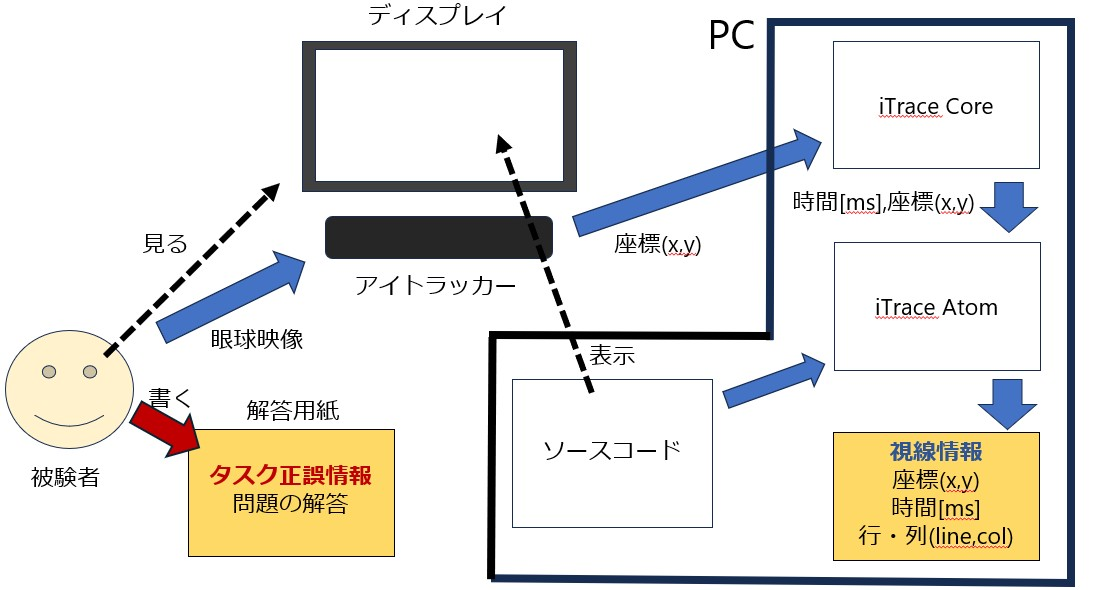
\includegraphics[width=0.8\linewidth]{実験装置全体図.jpg}
      \caption{実験装置の全体像}
    \end{figure}
    \FloatBarrier

    本章のまとめとして、図〇をもとに説明する。


\clearpage

\part{実験}
  本章では、実験の目的、実験に際し行った準備、当日の手順、得られたデータの概要を示す。\\

  \section{実験の目的}
    本実験は、以下の目的で行う。\\
    ・Javaの基礎知識を有する被験者が、複数のクラスで構成され100行以上にわたる比較的長大なJavaソースコードを読解する際の視線情報の収集\\
    ・上述のソースコード読解時の被験者のJava理解度の収集\\

    目的達成のため、以下の手段を用いる。\\
    ・被験者にソースコードと、それに対応するタスクを提示し、思考・解答中の視線座標をアイトラッカーを用いて収集し、視線情報とする\\
    ・被験者がタスクに正答した場合はソースコードを理解していると見なし、誤答した場合は理解していないと見なす\\


  \section{実験対象}
    実験は、近畿大学工業高等専門学校情報科4年生の学生33名を対象とする。被験者全員がオブジェクト指向を含むJavaプログラミングの授業を受講した経験がある。\\
    なお、被験者全員に以下の事項を伝え、承諾書にサインしてもらった。\\
    ・実験で使用する装置が身体に害を及ぼさないこと\\
    ・計測されたデータを個人を特定できないよう十分配慮した上で研究発表に使用すること\\
    ・被験者となるかは任意であり、実験結果が学校の成績等に一切の影響を与えないこと\\
    \\

  \section{被験者に提示するソースコードとタスク}
    \subsection{ソースコード}
      ソースコードはJavaで記述し、Mainクラスを含む計6つのクラスで構成されるものを準備する。
      コードは148行あり、上部にタスク3~5で使用するクラスが記述される。下部にはMainクラスが記述され、行で区切られた範囲に各タスクで使用する文が記述される。
      Mainクラス中に5つのタスクにまつわる記述を設けている。\\
      以下に、使用するソースコードの全体像を示す。
      \begin{figure}[h]
        \centering
        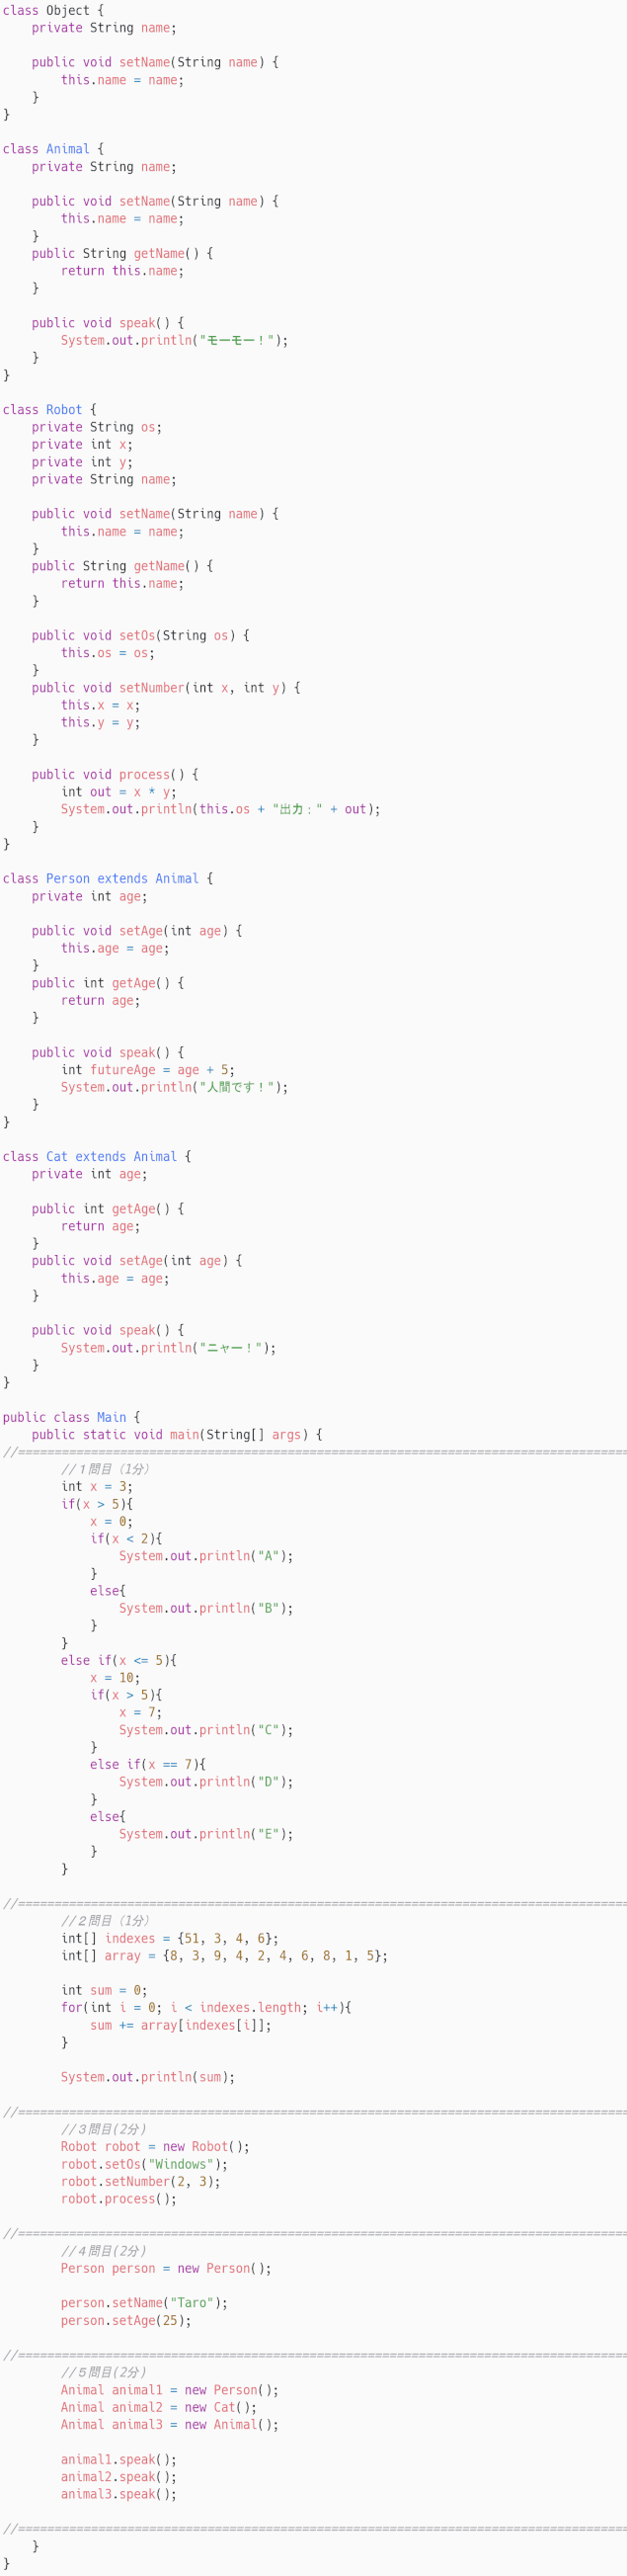
\includegraphics[height=\textheight]{carbon_clip_resized.png}
        \caption{使用するソースコード}
      \end{figure}
      \FloatBarrier

  \subsection{タスク}
    タスクは全5問用意する。うち2問がオブジェクト指向の概念を伴わないMainクラス内で完結するタスク、うち3問がオブジェクト指向の概念を伴うタスクである。
    以下にタスクの詳細を示す。\\
    \begin{enumerate}[label=タスク\arabic*:]
      \item 変数代入とif文による条件分岐を組み合わせたタスク。標準出力の出力結果を答えさせる。オブジェクト指向の概念を伴わない。
      \begin{figure}[h]
        \centering
        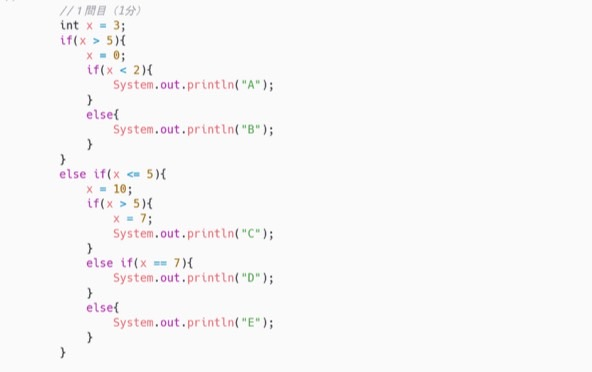
\includegraphics[height=0.5\linewidth]{プログラム画像_タスク1.jpg}
        \caption{タスク1のソースコード}
      \end{figure}
      \FloatBarrier
      \item 配列の参照を使用したタスク。標準出力の出力結果を答えさせる。オブジェクト指向の概念を伴わない。
      \begin{figure}[h]
        \centering
        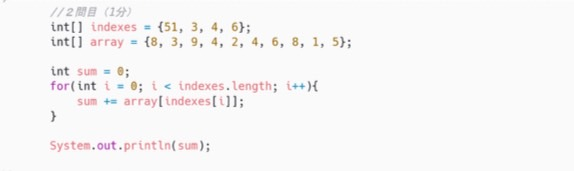
\includegraphics[height=0.25\linewidth]{プログラム画像_タスク2.jpg}
        \caption{タスク2のソースコード}
      \end{figure}
      \FloatBarrier
      \item 1種類のクラスを使用し、オブジェクト生成と外部からのメソッド実行を含むタスク。標準出力の出力結果を答えさせる。オブジェクト指向の概念を伴う。
      \begin{figure}[h]
        \centering
        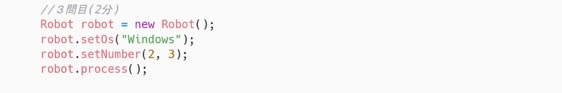
\includegraphics[height=0.2\linewidth]{プログラム画像_タスク3.jpg}
        \caption{タスク3のソースコード}
      \end{figure}
      \FloatBarrier
      \item 2種類のクラスを使用し、オブジェクト生成とセッターの呼び出しを含むタスク。2種類のクラスは片方がもう片方を継承する関係にある。
      ソースコード内で、それぞれのオブジェクトのセッターが定義された行を答えさせる。オブジェクト指向の概念を伴う。
      \begin{figure}[h]
        \centering
        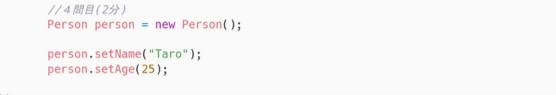
\includegraphics[height=0.2\linewidth]{プログラム画像_タスク4.jpg}
        \caption{タスク4のソースコード}
      \end{figure}
      \FloatBarrier
      \item 3種類のクラスを使用し、メソッドのオーバーライドを含む。標準出力の出力結果を答えさせる。オブジェクト指向の概念を伴う。
      \begin{figure}[h]
        \centering
        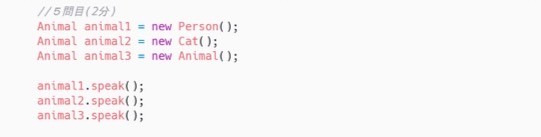
\includegraphics[height=0.25\linewidth]{プログラム画像_タスク5.jpg}
        \caption{タスク5のソースコード}
      \end{figure}
      \FloatBarrier
    \end{enumerate}

  \section{実験台の構成}
  本実験では、1つの実験台につき一人を座らせ、視線運動の測定を行う。
  実験台は3台用意する。各実験台の構成を以下に示す。\\
  ・ディスプレイ\\
  ・アイトラッカー\\
  ・顎台\\
  ・解答用紙\\
  ・PC\\

  実験台は、各回ごとにセットアップし、初期状態に戻す。

  \begin{figure}[h]
    \centering
    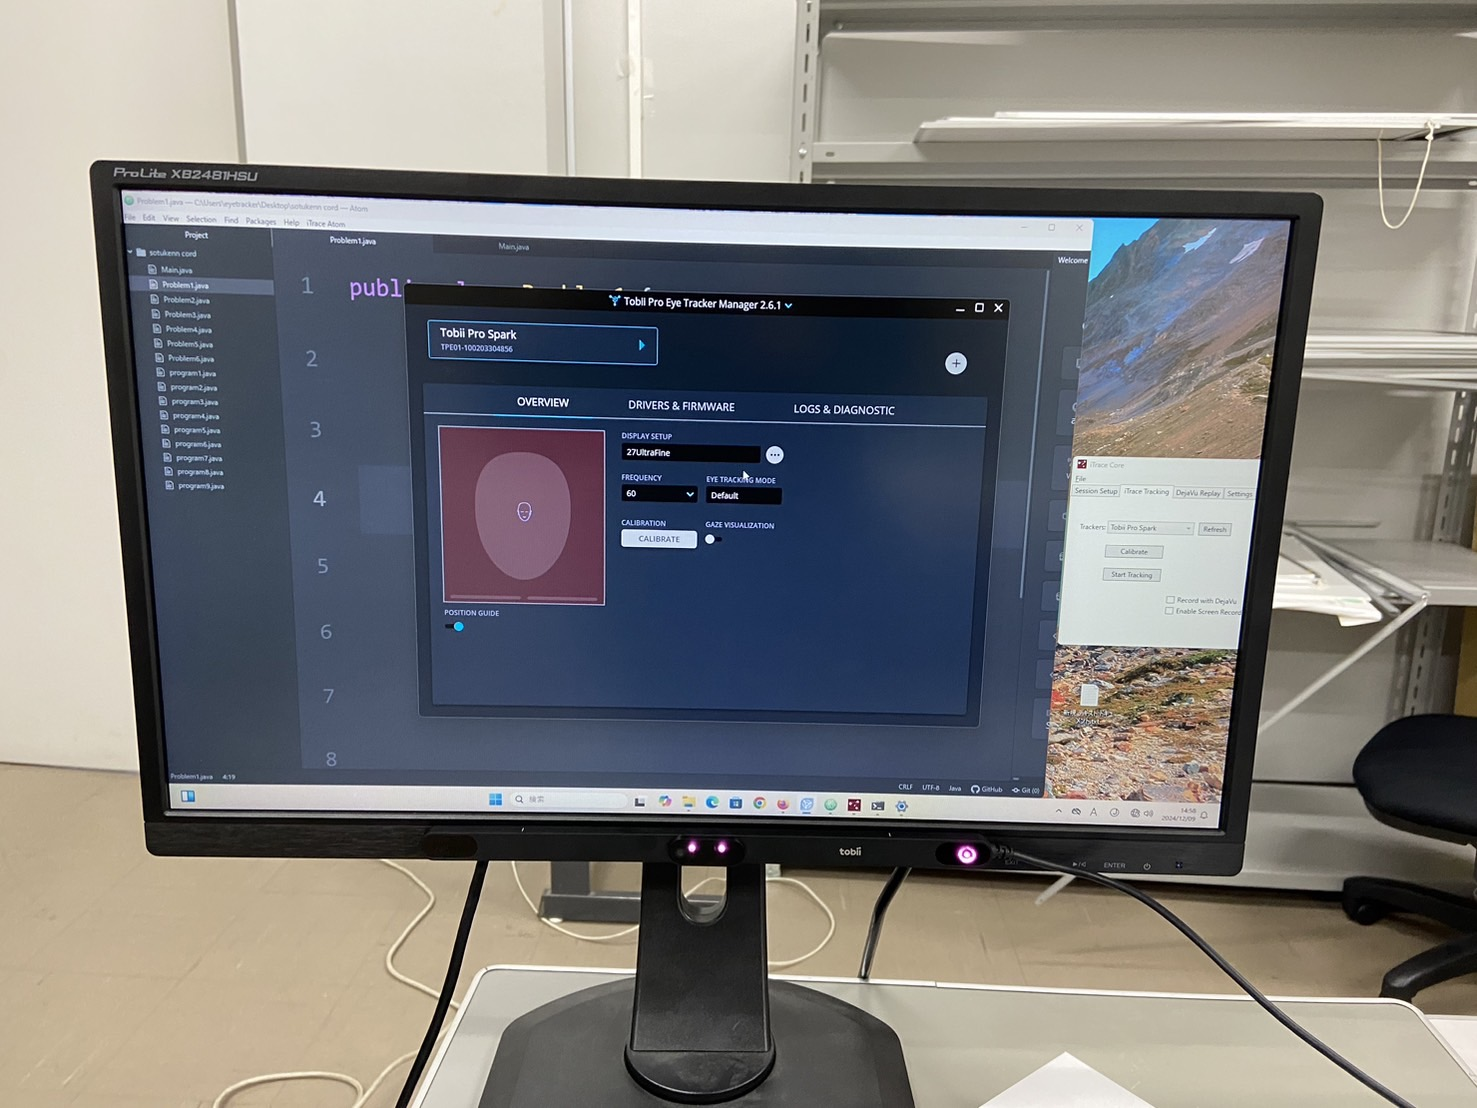
\includegraphics[height=0.5\linewidth]{実験台.jpg}
    \caption{初期状態のディスプレイの様子}
  \end{figure}
  

  \section{実験手順}
    実験は、以下の手順で行う。
    \begin{enumerate}
      \item 実験台のセットアップ
      \item 解答用紙への氏名記入・承諾書記入
      \item キャリブレーション
      \item 実験の流れの説明
      \item 練習問題
      \item 5つのタスク提示・視線座標計測
    \end{enumerate}
  

  \section{実験に使用する物品}
    実験に際して、以下の物が必要となる。
    \begin{enumerate}
      \item アイトラッカー
      \item アイトラッカーの設定・キャリブレーションに用いるソフトウェア(Tobii Pro Eye Tracker Manager)
      \item アイトラッカーの処理を担当するソフトウェア(iTrace Core)
      \item タスクに使用するソースコードを表示するエディタ(Atom)
      \item アイトラッカーで取得した画面上での座標を、ソースコードの行・列に変換する為のプラグイン
    \end{enumerate}
    以下、これらの物を解説する。

    \subsection{アイトラッカー}
      視線運動をディスプレイ画面上の時系列座標データとして取得するため,アイトラッカーと呼ばれる装置を使用する.本研究では,3台のディスプレイで同時に測定するため、計3台のアイトラッカーを準備する。
      内訳として、Tobii Pro Spark\cite{spark}2台とTobii Pro Nano\cite{nano}1台を使用する。
      \\
      Tobii Pro Spark、Tobii Pro Nanoともにディスプレイ装置の下部に固定することで,ディスプレイ画面上における被験者の注視点の座標を計測できる.
      サンプリングレートはいずれも60Hzである.測定の際,各被験者ごとにキャリブレーションする.

    \subsection{Tobii Pro Eye Tracker Manager}
      アイトラッカーのパラメータ設定、キャリブレーションにはTobii公式で提供されているTobii Pro Eye Tracker Managerというソフトウェアを使用する。
    
    \subsection{アイトラッカーの処理を担当するソフトウェア}
      アイトラッカーの測定開始・終了処理や、出力データの成型などを担当するソフトウェアとしてiTrace Core\cite{itrace}を使用する。

    \subsection{タスクに使用するソースコードを表示するエディタ(Atom)}
      エディタは、iTraceプラグインとの互換性のため、Atom\cite{atom}を使用する。

    \subsection{iTrace-Atomプラグイン}
      iTraceの出力座標データとエディタの画面表示情報を結びつけ、座標からプログラム中の行・列に対応させるため、Atomエディタのプラグインが開発されている。\\
      本研究では、Github上で公開されているiTrace-Atomプラグインに機能を追加したものを用いる。
    
      
    \subsection{ディスプレイ}
      画面サイズ1920×1200ピクセルのディスプレイを使用する。

    \subsection{コンピュータ}
      Windows11がセットアップされたコンピュータを使用する。


  \section{実験}
    3台の実験台を用い、3人ずつ同時並行で測定する。実験の流れを以下に示す。\\
    
    承諾書にサインしてもらう
    解答用紙に、出席番号と名前を書いてもらう
    3台の実験台それぞれに座ってもらい、キャリブレーションを行う。
    実験の流れの説明。
    ソースコードを読んで問題を解くこと、その際の視線データを計測すること、
    スクロール操作のみ行い、コードへの書き込みを行わないこと、回答がわかり次第挙手で合図し、解答用紙に書き込むこと、


    \begin{figure}[htbp]
      \centering
      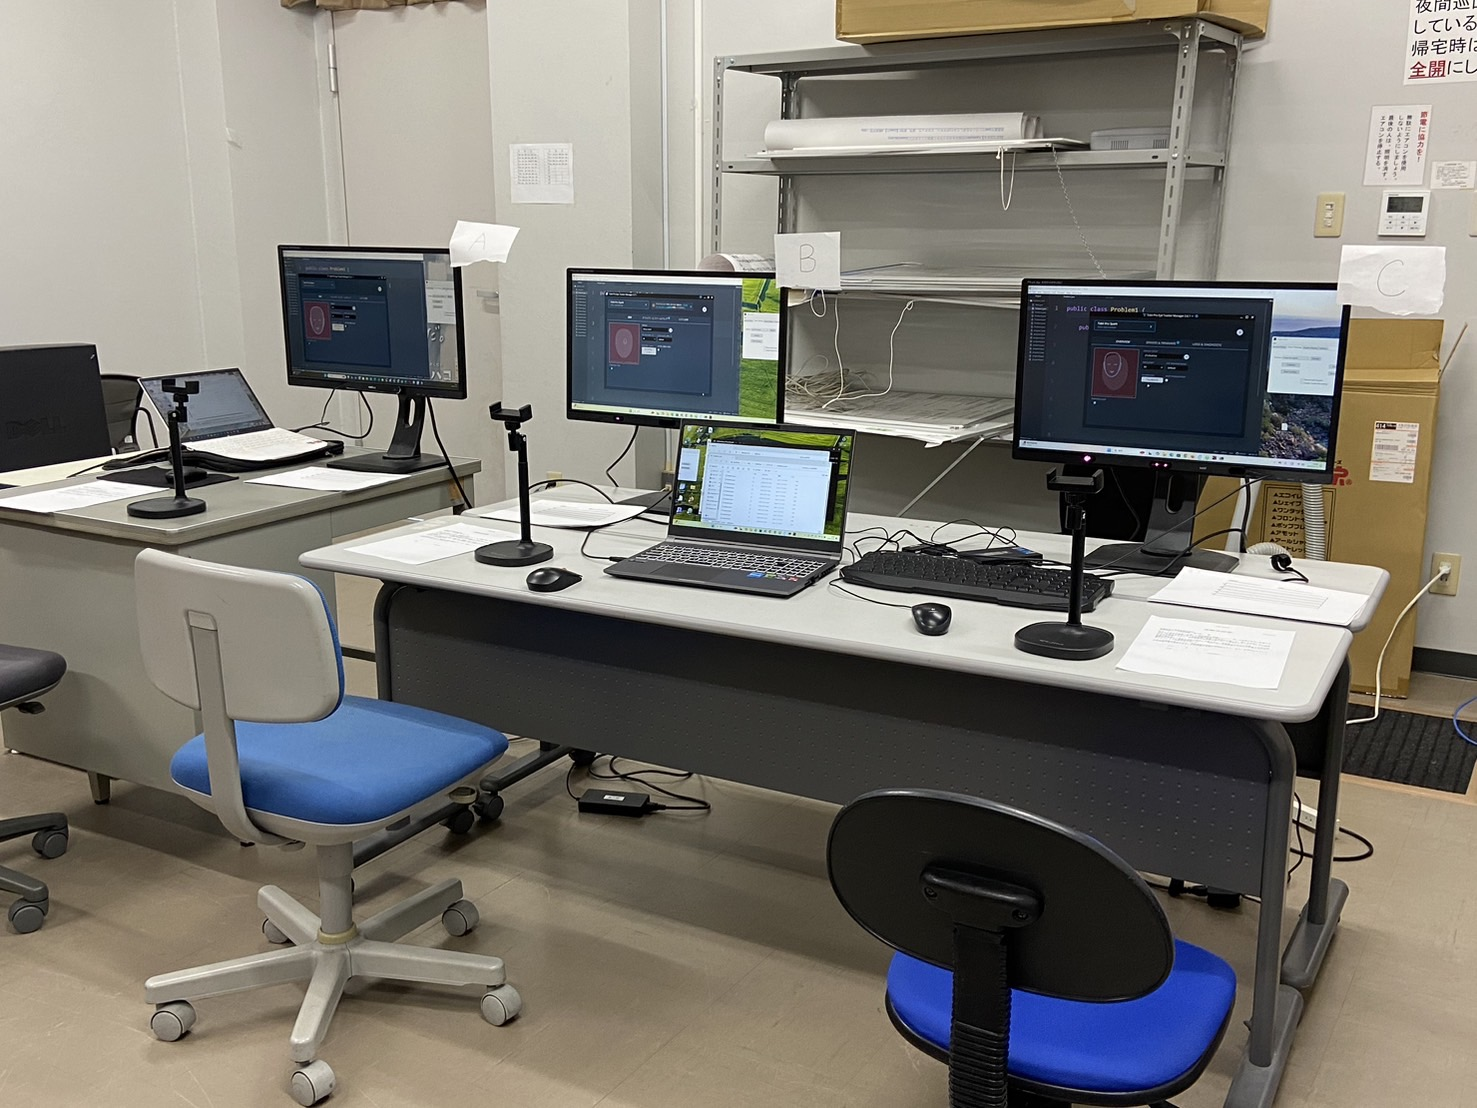
\includegraphics[width=0.8\linewidth]{実験部屋.jpg}
      \caption{実験部屋の様子}
    \end{figure}
    \FloatBarrier
  
  \section{実験結果}
    実験により、33人の視線座標データを取得した。そのうち、正確に保存されなかったデータと測定時のプログラムに誤りがあったデータを除き、
    後の分析に使用できるデータを抽出する。抽出後のタスクごとのデータ数と、正誤数を以下に示す。
    なお、タスク5において、3つある解答のうち、それぞれの内容はあっているものの記述順が異なっている場合に「惜しい」判定とした。\\
    \begin{table}[h]
      \centering
      \caption{実験により取得された使用可能データと、各タスクごとの正誤数}
      \begin{tabular}{|c|c|c|c|c|}
        \hline
        タスク名&使用可能なデータ数&正答数&誤答数&惜しい\\ \hline
        タスク1&26&6&20&-\\ \hline
        タスク2&10&3&7&-\\ \hline
        タスク3&10&3&7&-\\ \hline
        タスク4-1&26&2&24&-\\ \hline
        タスク4-2&26&7&19&-\\ \hline
        タスク5&26&13&8&5\\ \hline
      \end{tabular}
      \label{tab:basic}
    \end{table}
   \FloatBarrier


\clearpage

\part{データの分析}
  本章では、実験で得られたデータを加工し、クラスごとの注視時間割合に変換する過程と、その後の分析の一連の流れを示す。

  \section{はじめに}
    加工・分析の流れを以下に示す。\\

    生データxml→変数付きcsv→注視時間割合→主成分分析・3Dプロット描画

  \section{生データxml→変数付きcsv→注視時間割合}
   実験により得られた生データはxml形式で保存される。以下に、生データが持つパラメータを記す。\\
    \begin{table}[h]
      \centering
      \caption{生データに含まれるデータ一覧}
      \begin{tabular}{|c|c|c|}
        \hline
        パラメータ名 & 値の意味 & 値の例 \\ \hline
        screen\_width & ディスプレイ画面の横px数 & 1920 \\ \hline
        screen\_height & ディスプレイ画面の縦px数 & 1200 \\ \hline
        plugin\_type & プラグインの種類 & ATOM \\ \hline
        gaze & 視線情報 & 後述 \\ \hline
      \end{tabular}
      \label{tab:basic}
    \end{table}
   \FloatBarrier

   gazeパラメータはアイトラッカーのサンプリング数だけ存在し、それぞれ以下のパラメータを持つ。
  なお、アイトラッカーのサンプリングレートはTobii Pro Spark、Tobii Pro Nanoともに60Hzである。

  \begin{table}[h]
    \centering
    \caption{生データに含まれる視線情報}
    \begin{tabular}{|c|c|c|}
        \hline
        パラメータ名 & 値の意味 & 値の例 \\ \hline
        event\_id & 2 & 133784518694431017 \\ \hline
        plugin\_time & サンプリングのUNIX時間[ms] & 1733978269442 \\ \hline
        x & ディスプレイ画面上のx座標[px] & 480 \\ \hline
        y & ディスプレイ画面上のy座標[px] & 418 \\ \hline
        source\_file\_line & ソースコード中の行 & 2 \\ \hline
        source\_file\_col & ソースコード中の列 & 9 \\ \hline
        word & 視線が位置していた単語 & int \\ \hline
        gaze\_target & 視線が位置していたファイルの名前 & Problem1.java \\ \hline
        gaze\_target\_type & 対象ファイルの拡張子 & java \\ \hline
        source\_file\_path & 対象ファイルのファイルパス & Problem1.java \\ \hline
        editor\_line\_height & エディタの行の高さの設定値 & 40 \\ \hline
        editor\_font\_height & エディタのフォントサイズの設定値 & 120 \\ \hline
    \end{tabular}
    \label{tab:basic}
  \end{table}
  \FloatBarrier
  
  上述の生データから特定の情報を抜き出し、プログラムで扱いやすいようcsvに加工する。
  この際、サンプリング間の速度とAOI(Area Of Instance)も計算し、csvの列に加える。計算後の変数付きcsvの主なパラメータを以下に示す。
  \begin{table}[h]
    \centering
    \caption{変数付きcsvの主なパラメータ}
    \begin{tabular}{|c|c|c|}
        \hline
        パラメータ名 & 値の意味 & 値の例 \\ \hline
        time & 計測開始からの経過時間[ms] & 123 \\ \hline
        x & ディスプレイ画面上のx座標[px] & 480 \\ \hline
        y & ディスプレイ画面上のy座標[px] & 418 \\ \hline
        line & ソースコード中の行 & 2 \\ \hline
        col & ソースコード中の列 & 9 \\ \hline
        velocity & 速さ[px/ms] & 0.5893286\\ \hline
        AOI & クラス番号 & 1\\ \hline
    \end{tabular}
    \label{tab:basic}
  \end{table}
  \FloatBarrier


  求めた変数付きcsvから、クラスごとの注視時間割合を算出する。

  \section{注視時間割合の主成分分析}
  3Dプロットでの可視化のため、注視時間割合を主成分分析で3次元まで落とす。
  
  タスクの正誤で色分けして3Dプロットで可視化する。
  
  \section{3Dプロットの観察}
    \begin{figure}[htbp]
      \centering
      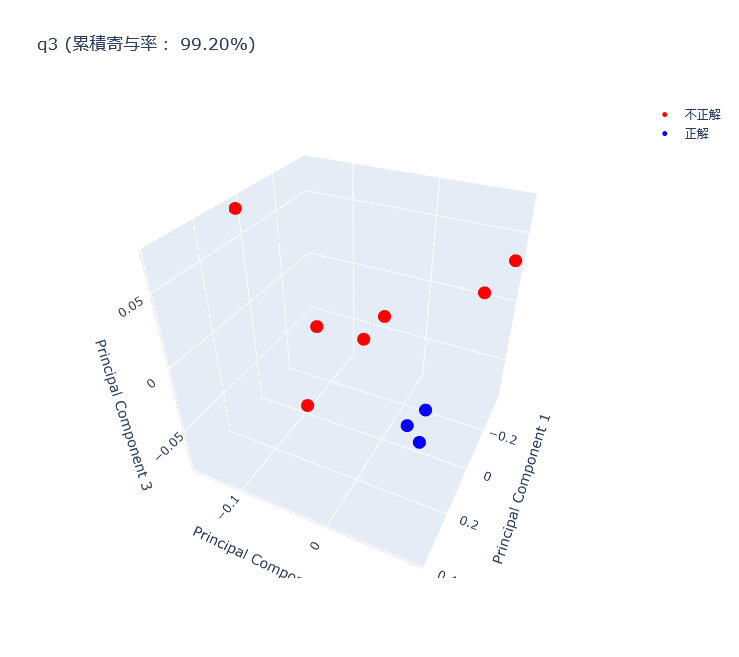
\includegraphics[width=0.8\linewidth]{3dplot_q3.png}
      \caption{タスク3の分布}
    \end{figure}
    \FloatBarrier
    \begin{figure}[htbp]
      \centering
      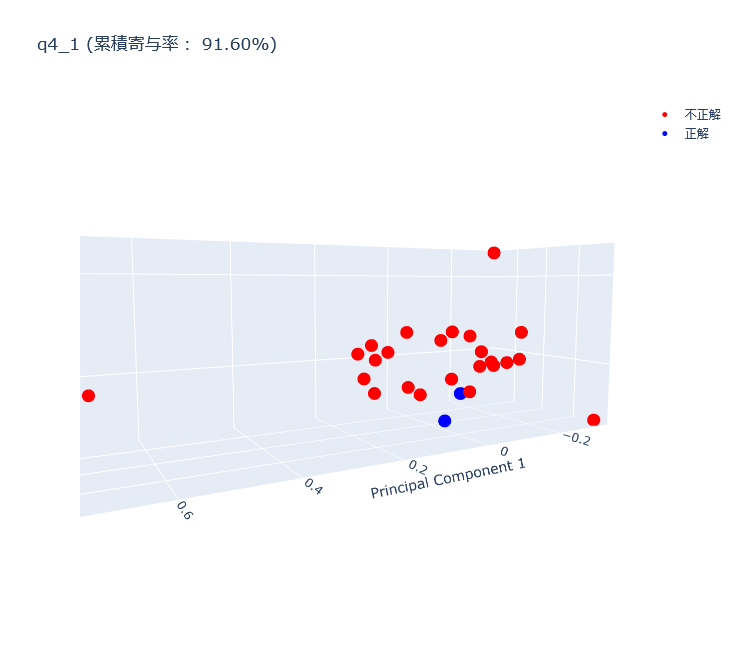
\includegraphics[width=0.8\linewidth]{3dplot_q4_1.png}
      \caption{タスク4-1の分布}
    \end{figure}
    \FloatBarrier
    \begin{figure}[htbp]
      \centering
      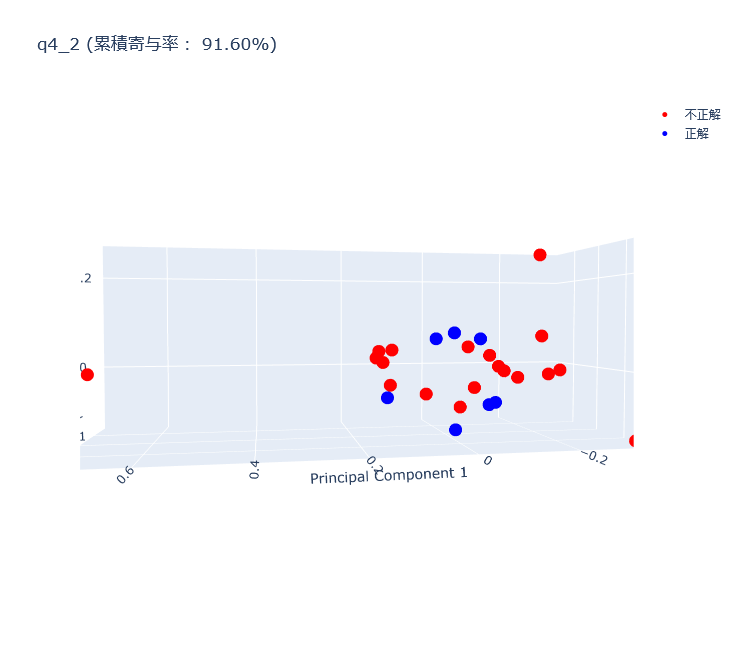
\includegraphics[width=0.8\linewidth]{3dplot_q4_2.png}
      \caption{タスク4-2の分布}
    \end{figure}
    \FloatBarrier
    \begin{figure}[htbp]
      \centering
      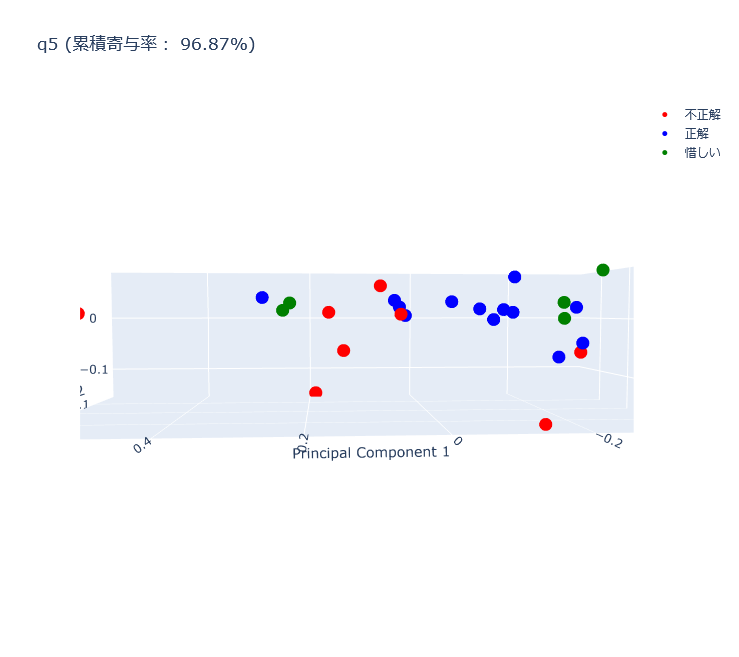
\includegraphics[width=0.8\linewidth]{3dplot_q5.png}
      \caption{タスク5の分布}
    \end{figure}
    \FloatBarrier

    タスク5を除くタスクにおいて、正答者のプロットが不正解者のものと比較して固まって位置していることが分かる。
    また、タスク5においても、正解者と不正解者で異なる分布になっていることが分かる。

\clearpage

\part{結論}
本研究により、オブジェクト指向を取り入れたタスクにおいて、正答者の視線運動は3次元グラフ上のある一定の範囲に固まる傾向があり、
不正答者のものはよりばらつきが大きいことが分かった。主成分分析での次元圧縮の際に算出した累積寄与率は90%以上と高く、
圧縮前のパラメータでもおおむね同様の傾向であるといえる。このことから、オブジェクト指向を取り入れたソースコードを用いたタスクにおいても
プログラミング理解度に応じて視線運動に差異が生じていることが分かった。
今後は、より多くのデータを集めて正答者の視線運動の傾向をつかみ、
その傾向から外れている場合に読解者がコードを理解していない可能性を検知できることが示唆された。

\pagebreak

\part*{謝辞}
本研究は,
大阪公立大学情報学研究科・情報処理領域の大野修一先生,
所属の岩佐英彦先生,
近畿大学工業高等専門学校情報科5年生の岡村晏志様、
および視線情報測定に協力して頂いた近畿大学工業高等専門学校・情報科4年生27名の協力により得られた成果である.ここに記して謝意を表します.

\pagebreak

\begin{thebibliography}{99}
  \bibitem{syougaku_program} 文部科学省,"小学校プログラミング教育の手引(第三版)",文部科学省,\url{https://www.mext.go.jp/a_menu/shotou/zyouhou/detail/1375607.htm},(参照:2025-2-13)
  \bibitem{tusuto_mondai} 大学入試センター,"情報 サンプル問題",文部科学省,\url{https://www.mext.go.jp/content/20211014-mxt_daigakuc02-000018441_9.pdf},(参照:2025-2-13)
  \bibitem{meiji2021} 泰地 酒井, 昌一 浦野,視線分析の傾向分析による特徴抽出,人工知能学会全国大会論文集,2021
  \bibitem{hanafusa} 亮 花房, 慎平 松本, 雄介 林, 宗 平嶋,視線運動を用いたプログラム読解パターンのデータ依存関係に基づく分析
  ーー代入演算と算術演算で構成されるプログラムを対象としてーー,教育システム情報学会誌,2018
  \bibitem{uwano} 吉岡春彦,上野秀剛,構文木と視線移動の自動マッピング手法を用いたプログラム理解過程の分析,ソフトウェアエンジニアリングシンポジウム2023,2023
  \bibitem{spark} Tobii Pro Spark https://www.tobii.com/ja/products/eye-trackers/screen-based/tobii-pro-spark
  \bibitem{nano} Tobii Pro Nano https://www.tobii.com/ja/products/discontinued/tobii-pro-nano
  \bibitem{manager} Tobii Pro Eye Tracker Manager https://connect.tobii.com/s/etm-download
  \bibitem{itrace} iTrace https://www.i-trace.org/
  \bibitem{atom} ATOM https://atom-editor.cc/
\end{thebibliography}


\end{document}
